\documentclass[10pt]{extarticle}
%Some packages I commonly use.
\usepackage[english]{babel}
\usepackage{graphicx}
\usepackage{framed}
\usepackage[normalem]{ulem}
\usepackage{amsmath}
\usepackage{amsthm}
\usepackage{amssymb}
\usepackage{amsfonts}
\usepackage{enumerate}
\usepackage[utf8]{inputenc}
\usepackage[top=1 in,bottom=1in, left=1 in, right=1 in]{geometry}

\title{Comparing per freq beam \& per coarse band beam}
\author{Wenyang Li}
\date{March 2019}

\begin{document}

\maketitle

\section{Introduction}
In this memo I tested different beam settings for the keyword nfreq\_avg in FHD-eppsilon pipeline and see if they make significant difference in the power spectra. It is of course correct to use per frequency beam in the analysis. However, it is computationally expensive, both in memory and time, to calculate per frequency channel beam. Using per coarse channel beam or per half coarse channel beam is much more computationally efficient but less robust. The reason to do this test is trying to see if using a lower frequency resolution beam introduces significant error and if it is worth the time and computation resources to calculate per frequency channel beam. The data I test on come from MWA Phase II zenith observations in 2016, containing 153 observations. I compared per frequency channel beam (80kHz resolution) setting and per half coarse channel beam (640kHz resolution) setting in my test. To simplify, I will call per frequency channel beam setting as the `\textbf{fiducial setting}', and the per half coarse setting as the `\textbf{cheap setting}'.

\section{Calibration}
The calibration was done in 40kHz resolution (768 channels). I compared calibration runs with fiducal setting and cheap setting when generating model visibilities. Figure \ref{fig:raw_cal}, \ref{fig:fit_cal} and \ref{fig:diff_cal} show the calibration comparison in these two cases. The difference between the two cases is at the level of $10^{-4}$. This shows that using a low resolution beam down to per 640kHz introduces negligible differences in calibration. One of the reason is that the FHD keyword `model\_delay\_filter' was on and it washes out some artifacts that a low resolution beam introduces.


\begin{figure}
    \centering
    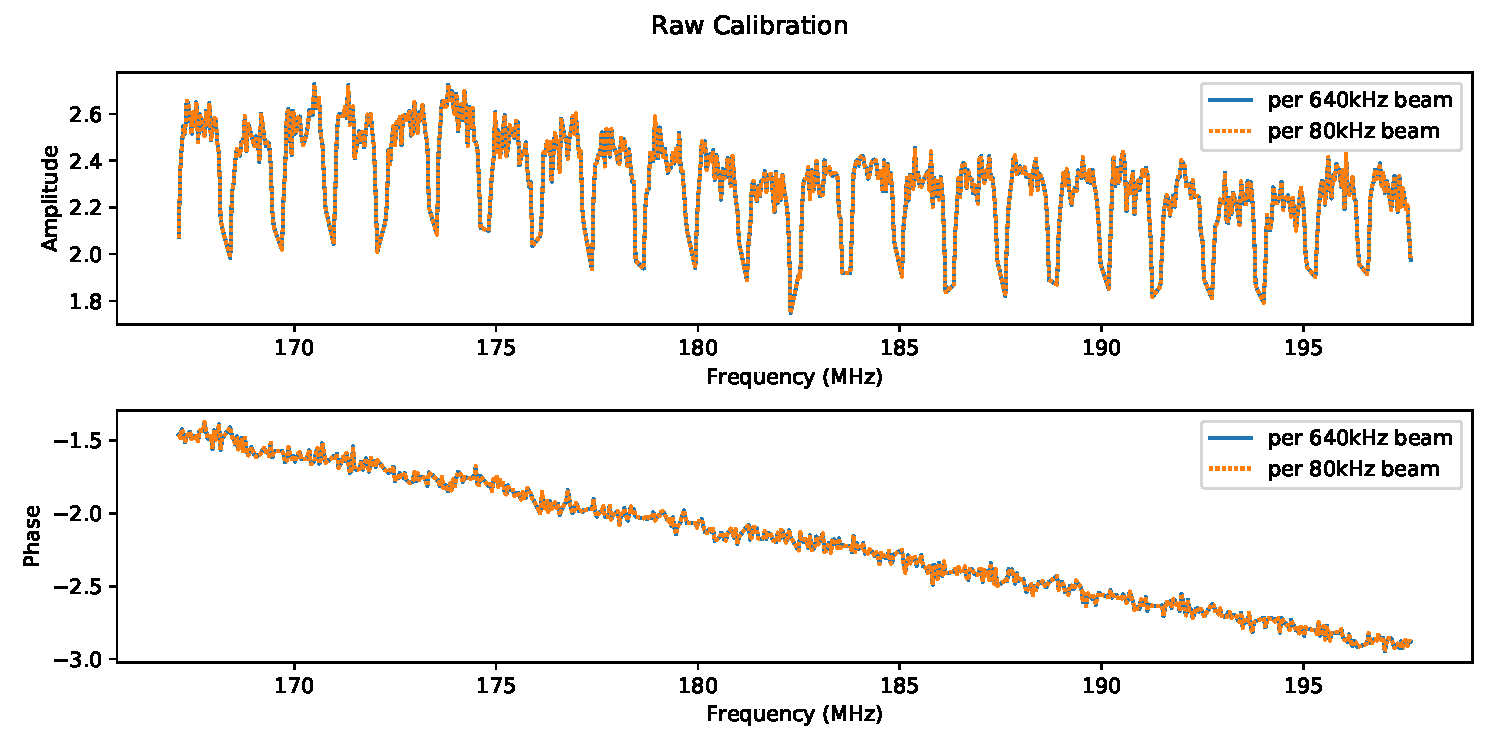
\includegraphics[width=0.8\linewidth]{raw_cal.pdf}
    \caption{Comparison between raw calibration}
    \label{fig:raw_cal}
\end{figure}


\begin{figure}
    \centering
    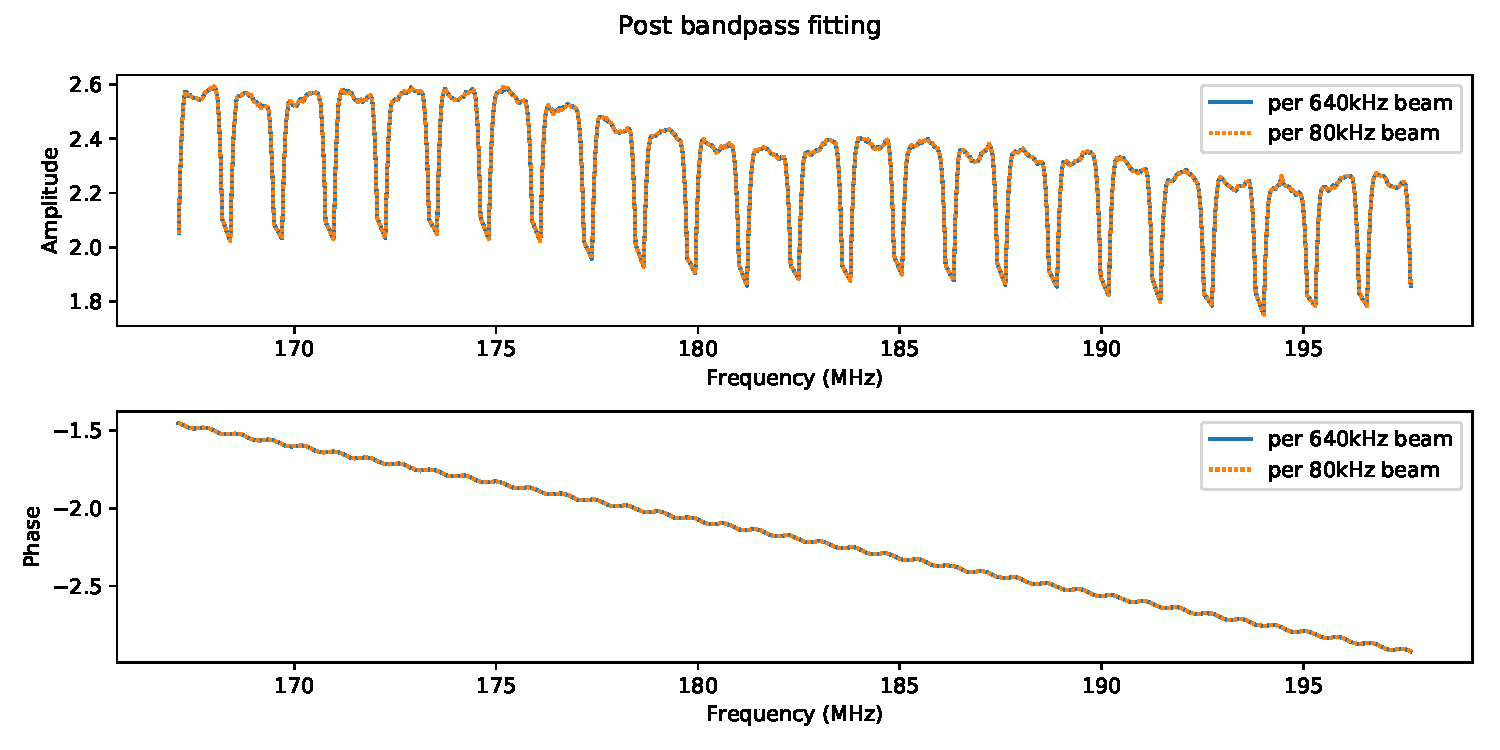
\includegraphics[width=0.8\linewidth]{fit_cal.pdf}
    \caption{Comparison between smoothed calibration}
    \label{fig:fit_cal}
\end{figure}

\begin{figure}
    \centering
    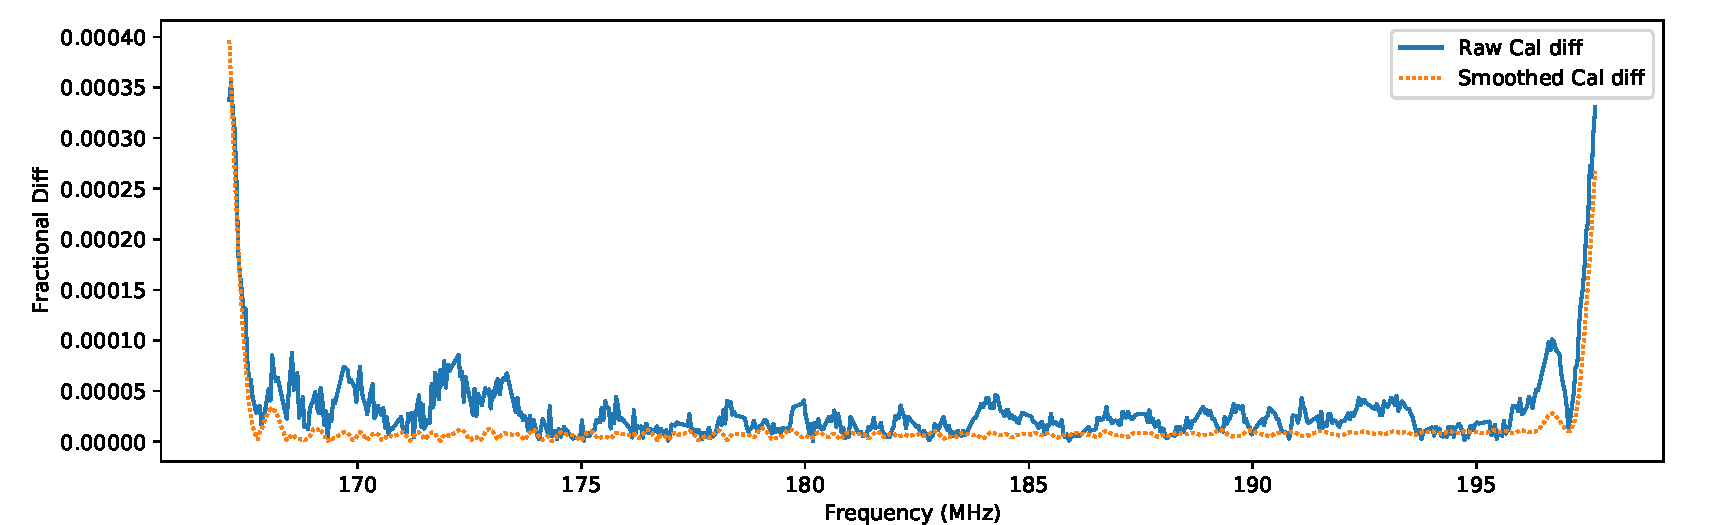
\includegraphics[width=0.8\linewidth]{diff_cal.pdf}
    \caption{Difference calibration}
    \label{fig:diff_cal}
\end{figure}

\begin{figure}
    \centering
    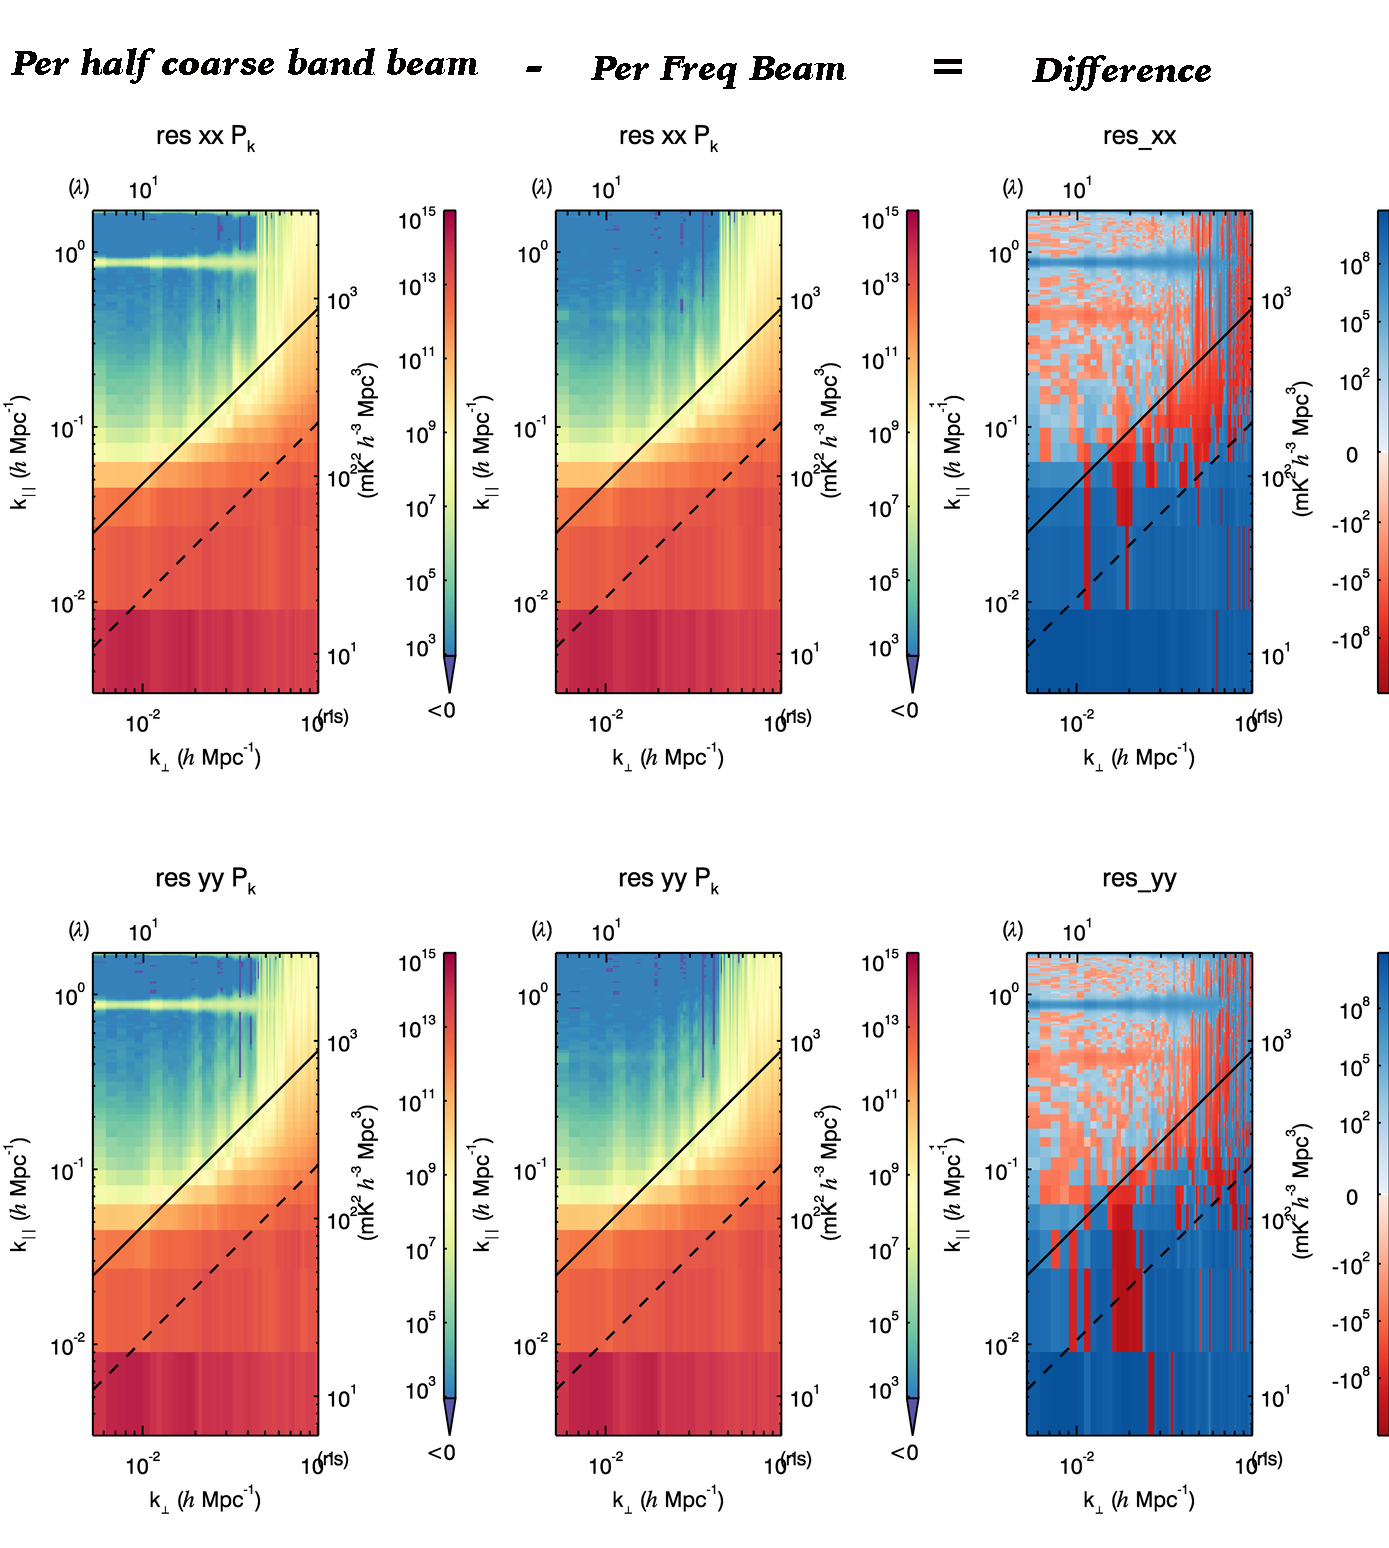
\includegraphics[width=\linewidth]{MODEL.png}
    \caption{Model ps comparison: left: per 640kHz beam; middle: 80kHz beam; right: left minus middle.}
    \label{fig:ps_model}
\end{figure}

\begin{figure}
    \centering
    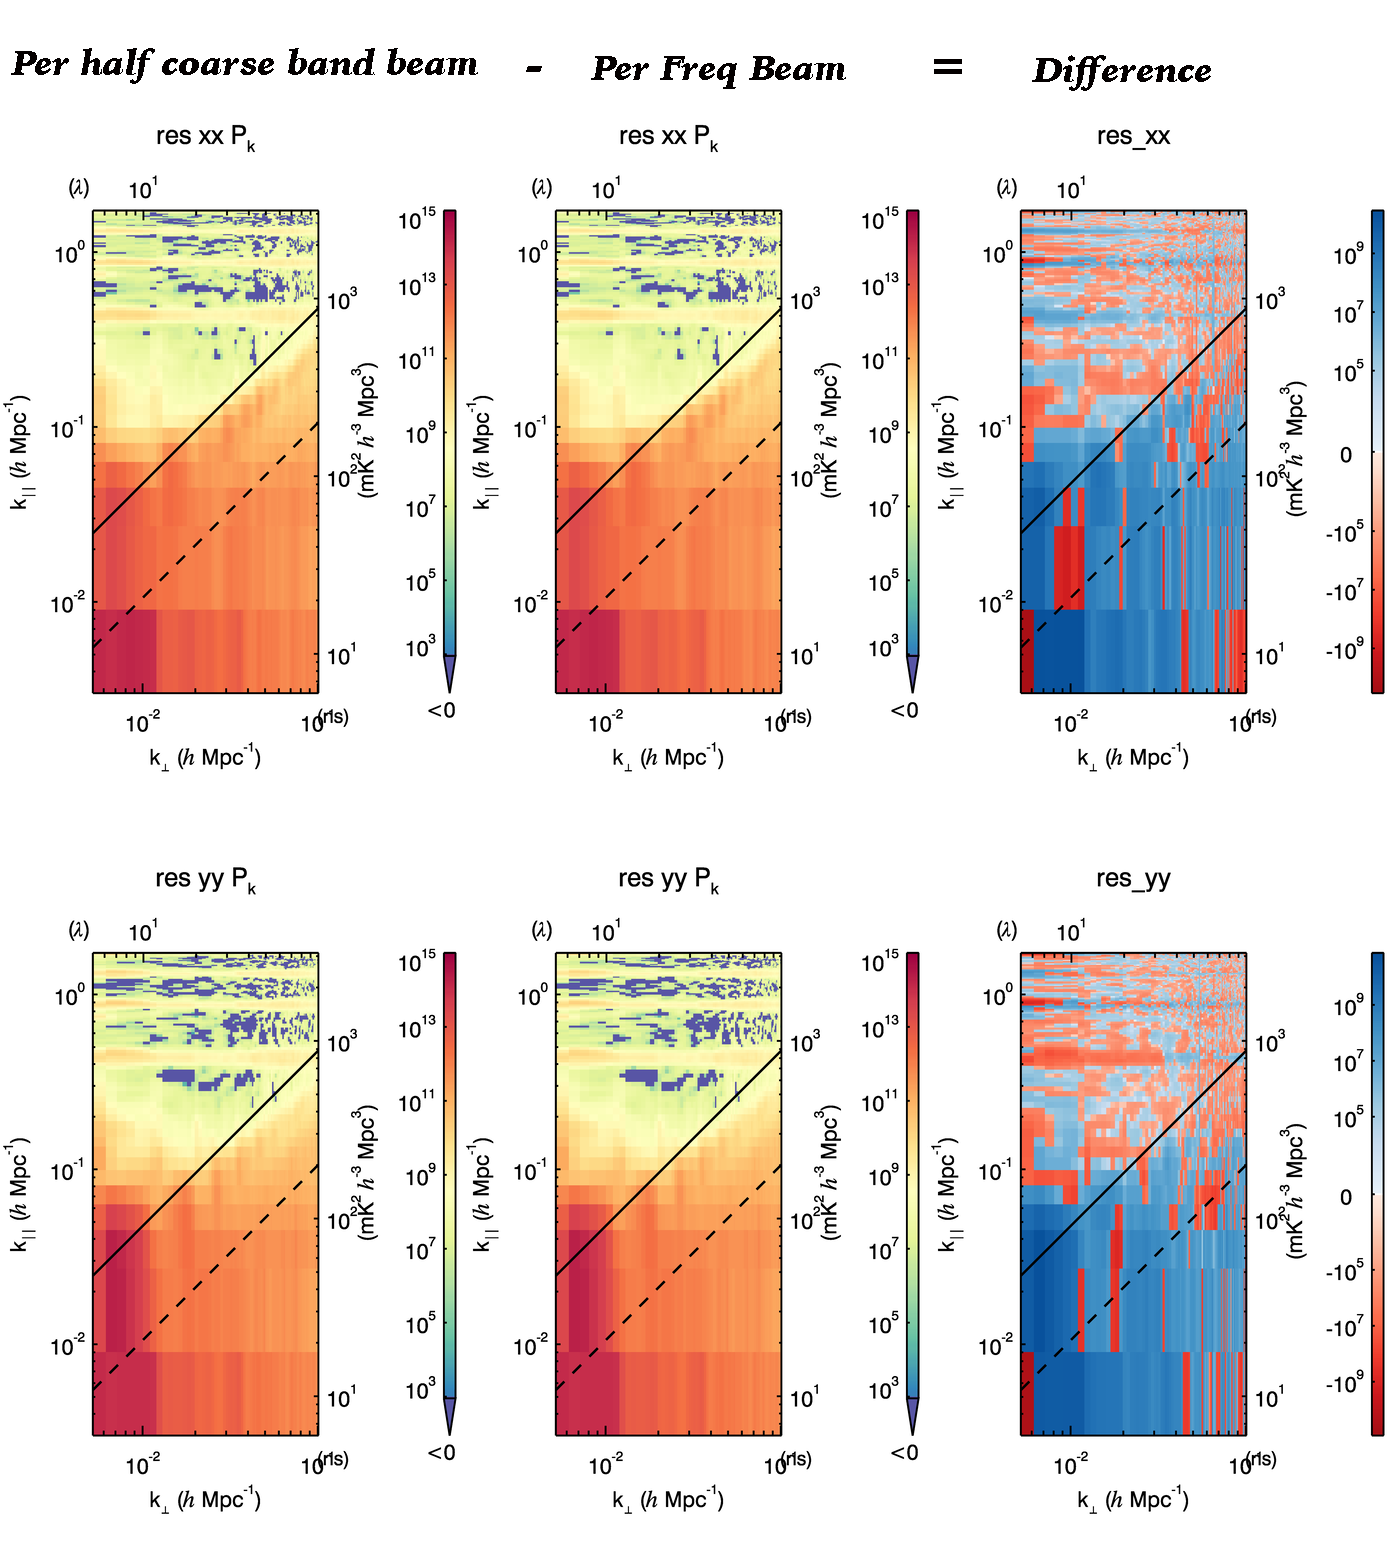
\includegraphics[width=\linewidth]{RESIDUAL.png}
    \caption{Residual ps comparison: left: per 640kHz beam; middle: 80kHz beam; right: left minus middle.}
    \label{fig:ps_res}
\end{figure}

\begin{figure}
    \centering
    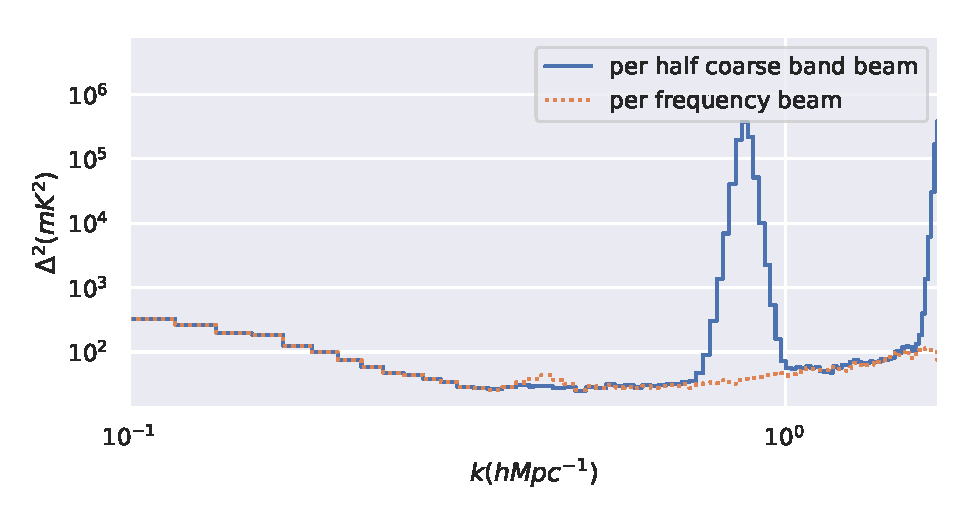
\includegraphics[width=\linewidth]{beam_ps_model.pdf}
    \caption{1d verison of model ps in Figure \ref{fig:ps_model}}
    \label{fig:model_1d}
\end{figure}

\begin{figure}
    \centering
    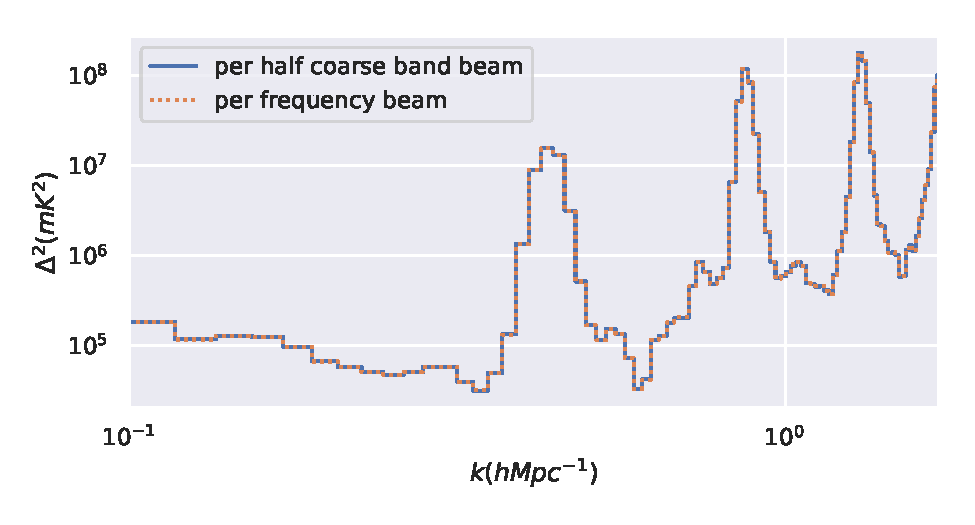
\includegraphics[width=\linewidth]{beam_ps_residual.pdf}
    \caption{1d version of residual ps in Figure \ref{fig:ps_res}}
    \label{fig:res_1d}
\end{figure}

\section{Model power spectrum}
To compare the differences in the model visibilities created by FHD used both for calibration and subtraction, I created model power spectrum for a single observation, with both the fiducial setting and the cheap setting. Figure \ref{fig:ps_model} shows that in the EoR window, the cheap setting only does harm to the second coarse band mode (because 640kHz corresponds to half of the coarse band), otherwise the power is unbiased in the EoR window. In the foreground wedge there is a bias, where the cheap setting introduces more power. This is understandable because the power is scaled less correctly for per half coarse band beam, especially at the edges of each half coarse band. The 1d comparison can be seen in Figure \ref{fig:model_1d}.


\section{Residual power spectrum}
The residual data is calculated by applying calibration solutions to the data, then subtract the model used for calibration from the data. This is done for both fiducial setting and cheap setting respectively. Now in the residual power spectrum analysis, the difference between the two runs are not only the calibration (although it is very small), but also the models being subtracted. To further compare the power spectrum, we also make the beam resolution consistent with the calibration settings, i.e., the residual from the cheap setting uses per 640kHz beam for healpix cube generation, and the residual from the fiducial setting uses per 80kHz beam for healpix cube generation. The 2d difference between these two cases is shown in Figure \ref{fig:ps_res}. The power in the window is still unbiased except for the coarse band modes. In the foreground wedge, same as the model ps difference shown in Figure \ref{fig:ps_model}, the cheap settings has more power, but with 3 factors contributing to it: 1. calibration being different; 2. the model subtracted being different; 3. the beam applied being different. The window power being unbiased indicates that it is safe to use per half coarse band beam for the whole analysis. Figure \ref{fig:res_1d} shows the 1d ps 2 sigma upper limit comparison. We can see that the power created in cheap setting and fiducial setting have negligible differences. 

\section{Conclusion}
In this memo I have tested using per 640kHz beam in the analysis, which is more computationally efficient but less robust, and compared it with the per frequency channel beam setting, which is reliable but computationally expensive. The results show that the less robust setting does not have significant error introduced the power spectrum. This gives us the confidence that we can use a more computationally efficient beam setting in our analysis without sacrificing the accuracy. I though stress that this memo only proves per 640kHz resolution or better is acceptable for MWA Phase II analysis, and the model delay filter has to be on. 

\end{document}